%            PACKAGES AND OTHER DOCUMENT CONFIGURATIONS
%----------------------------------------------------------------------------------------
\documentclass[paper=letter,8.5pt]{article}

\usepackage[spanish]{babel} 
\usepackage{amsmath,amsfonts,amsthm} % Math packages
\usepackage{floatrow}
\usepackage[utf8]{inputenc}
\usepackage{float}
\usepackage{lipsum} % Package to generate dummy text throughout this template
\usepackage{blindtext}
\usepackage{graphicx} 
\graphicspath{ {./Imágenes/} }
\usepackage[font=footnotesize,labelfont=bf]{caption}
\usepackage{subcaption}
\usepackage[sc]{mathpazo} % Use the Palatino font

\usepackage[T1]{fontenc} % Use 8-bit encoding that has 256 glyphs
\linespread{1.05} % Line spacing - Palatino needs more space between lines
\usepackage{microtype} % Slightly tweak font spacing for aesthetics
\usepackage[hmarginratio=1:1,top=32mm,columnsep=20pt]{geometry} % Document margins
\usepackage{multicol} % Used for the two-column layout of the document
%\usepackage[hang, small,labelfont=bf,up,textfont=it,up]{caption} % Custom captions under/above floats in tables or figures
\usepackage{booktabs} % Horizontal rules in tables
\usepackage{float} % Required for tables and figures in the multi-column environment - they need to be placed in specific locations with the [H] (e.g. \begin{table}[H])
\usepackage{hyperref} % For hyperlinks in the PDF
\usepackage{wrapfig}
\usepackage{xcolor}
\usepackage{lettrine} % The lettrine is the first enlarged letter at the beginning of the text
\usepackage{paralist} % Used for the compactitem environment which makes bullet points with less space between them
\usepackage{abstract} % Allows abstract customization
\renewcommand{\abstractnamefont}{\normalfont\bfseries} % Set the "Abstract" text to bold
\renewcommand{\abstracttextfont}{\normalfont\small\itshape} % Set the abstract itself to small italic text
\usepackage{titlesec} % Allows customization of titles

\renewcommand\thesection{\Roman{section}} % Roman numerals for the sections
\renewcommand\thesubsection{\Roman{subsection}} % Roman numerals for subsections
\newcommand{\uvec}[1]{\hat{e}_{#1}}

\titleformat{\section}[block]{\large\scshape\centering}{\thesection.}{1em}{} % Change the look of the section titles
\titleformat{\subsection}[block]{\large}{\thesubsection.}{1em}{} % Change the look of the section titles
\newcommand{\horrule}[1]{\rule{\linewidth}{#1}} % Create horizontal rule command with 1 argument of height


%cambiar a negrita los numeros de las ecuaciones
%\makeatletter
%\def\tagform@#1{\maketag@@@{(\ignorespaces\textbf{#1}\unskip\@@italiccorr)}}
%\renewcommand{\eqref}[1]{\textup{{\normalfont(\ref{#1}}\normalfont)}}
%\makeatother

%---------------------------------------------------------------------------------------
%IMÁGENES INCLUIDAS


%----------------------------------------------------------------------------------
\hypersetup{colorlinks=true,linkcolor=blue,citecolor=blue,filecolor=blue,urlcolor=magenta,}

\usepackage{fancyhdr} % Headers and footers
\pagestyle{fancy} % All pages have headers and footers
\fancyhead{} % Blank out the default header
\fancyfoot{} % Blank out the default footer


\fancyhead[RO,LE]{Universidad Nacional Autónoma de México | Facultad de Ciencias | Servicio Social } % Custom header text
\renewcommand{\headrulewidth}{0.4pt}

\fancyfoot[RO,LE]{\thepage} % Custom footer text
\fancyheadoffset[RO,LE]{0.01\textwidth}


%----------------------------------------------------------------------------------------
%       TITLE SECTION
%----------------------------------------------------------------------------------------
\title{\vspace{-15mm}\fontsize{17pt}\selectfont\textbf{Cálculo de las secciones transversales de extinción, absorción y esparcimiento de elipsoides en la aproximación cuasiestática como primera aproximación de eritrocitos }} % Article title
\author{
\large
{\textsc{ Dana Larissa Luna González}}\\[2mm]}
\date{}
\geometry{total={170mm,230mm}, left=20mm, top=25mm}
 
\begin{document}
\maketitle % Insert title
\thispagestyle{fancy} % All pages have headers and footers
\section{Introducción}
\subsection{Aproximación cuasiestática en el problema de esparcimiento de luz por partículas elipsoidales}

 En el caso de un elipsoide caracterizado por una función dieléctrica $\epsilon_p$, que se encuentra inmerso en un medio caracterizado por una función dieléctrica $\epsilon_m$ y cuyo semieje mayor es $a$, se puede definir el límite cuasiestático cuando el parámetro de tamaño $x=ka$ es mucho menor que la unidad \cite{Bohren}, donde $k=2\pi \sqrt{\epsilon_m}/\lambda$ con $\lambda$ la longitud de onda. Esta aproximación garantiza que toda la geometría del elipsoide esté sujeta a un campo eléctrico de la misma intensidad y dirección \cite{Miguel}. En esta sección se estudiará el caso del dipolo eléctrico de una esfera para introducir el concepto de polarizabilidad, y más adelante, se desarrollará el dipolo eléctrico para esparcidores arbitrarios en donde se analizarán las regiones de campo cercano, la intermedia y la de radiación.


\subsubsection{Dipolo eléctrico (caso estático)}

En electrodinámica clásica, se entiende como \textit{límite cuasiestático} el considerar una partícula de tamaño mucho menor que la longitud de onda de la luz incidente \cite{Cuasiest}. Para el caso de una partícula esférica, se puede emplear la aproximación cuasiestática al resolver la ecuación de Laplace para el potencial eléctrico $\phi$. En particular, esta solución deviene en \cite{Griffiths}:
\begin{equation}
\phi=\frac{p}{4\pi\epsilon_m}\left(\frac{\Vec{r}\cdot\hat{e}_z}{r^3}\right)=\frac{\Vec{p}\cdot\Vec{r}}{4\pi\epsilon_m r^3}=\frac{p\cos\theta}{4\pi\epsilon_m r^2}
\label{pot_dipolo}
\end{equation}
donde $\Vec{p}$ representa el momento dipolar eléctrico. Si se considera una esfera con permitividad eléctrica $\epsilon_p$, embebida en el mismo medio caracterizado por su función dieléctrica $\epsilon_m$ en el cual existe un campo eléctrico uniforme $\Vec{E}_0=E_0\hat{e}_z$, al resolver la ecuación de Laplace considerando las condiciones de frontera entre la esfera y el medio, se obtiene que el campo eléctrico fuera de la esfera es la superposición del campo eléctrico aplicado y del campo eléctrico producido por un dipolo eléctrico puntual localizado en el origen con momento dipolar \cite{Bohren}:
\begin{equation}
	\vec{p}= \epsilon_m\alpha\Vec{E}_0=4\pi\epsilon_m a^3\frac{\epsilon_1-\epsilon_m}{\epsilon_1+2\epsilon_m}\Vec{E}_0, \;\text{con}\; \alpha=4\pi a^3(\epsilon_1-\epsilon_m)/(\epsilon_1+2\epsilon_m),
	\label{momentdipol}
\end{equation}
donde $\alpha$ es la polarizabilidad eléctrica, que representa la facilidad con la que se polariza la esfera. Es decir, el campo eléctrico induce un dipolo eléctrico en la esfera.
\begin{figure}[h!]
	\includegraphics[width=6cm]{../../Figuras/shereE0}
	\caption{Esfera de radio $r$ caracterizada por su función dieléctrica $\epsilon_p$ y embebida en un medio caracterizado por su función dieléctrica $\epsilon_$ en la cual incide un campo eléctrico uniforme $\Vec{E}_0$.}
\end{figure}


\subsubsection{Dipolo eléctrico (caso dinámico)}}

En la sección anterior se abordó una solución que asume que el campo eléctrico,  por tanto el dipolo inducido, son estáticos. Para resolver el caso dinámico en el límite cuasiestático, se asume ahora que las cargas están localizadas en un volumen finito moviéndose en presencia de un campo eléctrico dinámico; lo cual es equivalente a realizar un análisis en componentes de Fourier de los potenciales y campos de un sistema de cargas y corrientes localizadas en el espacio vacío, con una dependencia armónica $e^{-i\omega t}$, tal que varían en el tiempo y oscilan a la frecuencia $\omega$ del campo electromagnético aplicado. De esta forma, la densidad volumétrica de carga $\rho(\Vec{r},t)$ y la densidad de corriente $\Vec{J}(\Vec{r},t)$  en la posición $\Vec{r}$ se expresan como \cite{Jackson}
\begin{align}
    \rho(\Vec{r},t)&=\rho(\Vec{r})e^{-i\omega t},\nonumber\\
    \Vec{J}(\Vec{r},t)&=\Vec{J}(\Vec{r})e^{-i\omega t},
    \label{armonicf}
\end{align}
considerando que el significado físico lo posee la parte real. Mediante lo anterior, es posible determinar los campos electromagnéticos mediante el potencial vectorial como \cite{Jackson}:
\begin{align}
  \Vec{A}(\Vec{r},t)=\frac{\mu_0}{4\pi}\int \text{d}^3r'\frac{\Vec{J}(\Vec{r'})e^{i\omega \frac{|\Vec{r}-\Vec{r'}|}{c}}}{|\Vec{r}-\Vec{r'}|}e^{-i\omega t_r},
  \label{Achafa}
\end{align}
en donde se emplea la norma de Lorentz \cite{Griffiths} y la densidad de corriente se evalúa en el tiempo de retardo $t_r=t-|\Vec{r}-\Vec{r'}|/c$. \\

El comportamiento de los campos electromagnéticos se puede estudiar al delimitar diferentes regiones considerando valores extremos de $k=\omega/c$, como se verá a continuación. Empleando la definición anterior y obviando la dependencia temporal, la Ec. (\ref{Achafa}) se reescribe como
\begin{equation}
    \Vec{A}(\Vec{r},t)=\frac{\mu_0}{4\pi}\int \Vec{J}(\Vec{r'})\frac{e^{ik|\Vec{r}-\Vec{r'}|}}{|\Vec{r}-\Vec{r'}|} \text{d}^3r'.
    \label{pot_vectorial}
\end{equation} 
En la región de campo cercano, donde $r\ll\lambda$ (o $kr\ll 1$), tal que exp($ik|\Vec{r}-\Vec{r'}|)\to 1$, se tiene \cite{Jackson}
\begin{equation*}
	\Vec{A}(\Vec{r},t)=\frac{\mu_0}{4\pi}\int \frac{\Vec{J}(\Vec{r'})}{|\Vec{r}-\Vec{r'}|} \text{d}^3r',
\end{equation*} 
mientras que en la región de campo lejano ($kr\gg 1$) dado que la exponencial oscila rápidamente, es suficiente aproximar
\begin{equation}
	|\Vec{r}-\Vec{r'}|\simeq r-\hat{e}_r\cdot\Vec{r'},    
\end{equation}
con $\hat{e}_r$ un vector unitario en la dirección de $\Vec{r}$. \footnote{Empleando la ley de cosenos y haciendo una expansión binomial $
	|\Vec{r}-\Vec{r'}|=\sqrt{r^2+(r')^2-2rr'\cos\theta}=r\sqrt{1+\left(r'/r\right)^2-2\left((r'/r)\cos\theta\right)}\simeq r\left\{1-(\hat{e}_r\cdot\Vec{r'}/r)+1/2\left(r'/r\right)^2\right\}\simeq r-\hat{e}_r\cdot\Vec{r'}.$} 	
	Si sólo se consideran los términos que decaen como $r^{-1}$, el inverso de la distancia en la Ec. (\ref{pot_vectorial}) puede ser reemplazado por $r$. Entonces, el potencial vectorial es
	\begin{equation*}
	\lim_{kr\rightarrow\infty}\Vec{A}(\Vec{r})=\frac{\mu_0}{4\pi}\frac{e^{ikr}}{r}\int \Vec{J}(\Vec{r'})e^{-ik\hat{e}_r\cdot\Vec{r'}}\text{d}^3r',    
	\end{equation*}
	que se puede reescribir al realizar la expansión en serie de potencias de la exponencial dentro de la integral de volumen, dando como resultado
	\begin{equation*}
	\lim_{kr\rightarrow\infty}\Vec{A}(\Vec{r})=\frac{\mu_0}{4\pi}\frac{e^{ikr}}{r}\sum_n\frac{(-ik)^n}{n!}\int \Vec{J}(\Vec{r'})(\hat{e}_r\cdot\Vec{r'})^n \text{d}^3r'.    
	\end{equation*}
\begin{figure}[h!]
	\includegraphics[width=6cm]{../../Figuras/aprox.jpg}
	\caption{Vector de posición $\Vec{r}$ del volumen y $\Vec{r'}$. Se muestra la distancia $|\Vec{r}-\Vec{r'}|$ entre estos últimos. }
\end{figure}
Al considerar únicamente el primer término de la expansión, se concluye que 
\begin{equation}
    \Vec{A}(\Vec{r})\approx\frac{\mu_0}{4\pi}\frac{e^{ikr}}{r}\int \Vec{J}(\Vec{r'}) \text{d}^3r',    
    \label{aprox_pot_vec}
\end{equation}
que al realizar una integración por partes,  \footnote{Al considerar $\int_V \Vec{r'}(\nabla'\cdot\Vec{J})\text{d}^3r'=\int_{\partial V} \Vec{r'}(\Vec{J}\cdot \text{d}\Vec{S})-\int_V \Vec{J}\text{d}^3r'$ y asumiendo que $\Vec{J}$ se desvanece en los límites del volumen $V$, es decir, en la superficie $\partial V$. } se obtiene que
\begin{equation}
	\int\Vec{J}d^3r'=-\int \Vec{r'}(\nabla'\cdot\Vec{J})\text{d}^3r'=-i\omega\int \Vec{r'}\rho(\Vec{r'})\text{d}^3r',
	\label{Jrho}
\end{equation}
donde se emplea la ecuación de continuidad
\begin{equation*}
    \nabla\cdot\Vec{J}=-\frac{\partial\rho}{\partial t}=i\omega\rho(\Vec{r}). 
\end{equation*}
Al sustituir la Ec. (\ref{Jrho}) en la Ec. (\ref{aprox_pot_vec}) y considerando que el momento dipolar eléctrico $\Vec{p}$ de una distribución de cargas $\rho$ es
\begin{equation*}
	\Vec{p}=\int \Vec{r'}\rho(\Vec{r'})\text{d}^3r',
\end{equation*}
se obtiene 
\begin{equation}
    \Vec{A}(\Vec{r})=-\frac{i\omega\mu_0}{4\pi}\frac{e^{ikr}}{r}\int \Vec{r'}\rho(\Vec{r'})\text{d}^3r'=-\frac{i\omega\mu_0}{4\pi}\frac{e^{ikr}}{r}\Vec{p}. 
    \label{A_dip}  
\end{equation}
Al calcular el campo $\Vec{H}$ como función del potencial vectorial, y empleando la ley de Faraday-Lenz para determinar el campo eléctrico, se concluye que \cite{Jackson}
\begin{align}
	\Vec{E}&=\frac{1}{4\pi\epsilon_0}\left\{k^2(\hat{e}_r\times\Vec{p})\times\hat{e}_r\frac{e^{ikr}}{r}+[3\hat{e}_r(\hat{e}_r\cdot\Vec{p})-\Vec{p}]\left(\frac{1}{r^3}-\frac{ik}{r^2}\right)e^{ikr}\right\},\label{E}\\
    \Vec{H}&=\frac{ck^2}{4\pi}(\hat{e}_r\times\Vec{p})\frac{e^{ikr}}{r}\left(1-\frac{1}{ikr}\right).    \label{H}
\end{align}
A partir de las Ecs. (\ref{E})  y (\ref{H}) se puede observar que el campo $\Vec{H}$ es transversal al vector radial para cualquier distancia, mientras el campo eléctrico tiene componentes paralelas y perpendiculares a $\hat{e}_r$.\\ 

 De forma análoga al desarrollo de la Ec. (\ref{A_dip}) y empleando la Ley de Faraday Lenz, en la zona de radiación cuando $kr\gg 1$, se tiene que al excitar a las fuentes en el sistema mediante una onda electromagnética de frecuencia angular $\omega$, lo que sería equivalente a iluminar al sistema con una onda plana armónica en el tiempo, se induce un dipolo eléctrico $\Vec{p}$ que genera campos electromagnéticos $\Vec{E}_p$ y $\Vec{H}_p$ y  que oscilan a la misma frecuencia $\omega$ 
\begin{align}
    \Vec{E}_p&=\frac{e^{ikr}}{-ikr}\frac{ik^3}{4\pi\epsilon_m}\hat{e}_r\times(\hat{e}_r\times \Vec{p}) e^{i\omega t}, \hspace{1cm}
    \Vec{H}_p=\frac{ck^2}{4\pi}(\hat{e}_r\times\Vec{p})\frac{e^{ikr}}{r}e^{i\omega t}.
\end{align}
En el caso particular en que el sistema se ilumine con una onda plana monocromática, es decir, de una sola frecuencia, y polarizada en la dirección $\hat{e}_x$, que induce un dipolo eléctrico con momento dipolar  $\Vec{p}=\epsilon_m \alpha E_0 e^{-i\omega t}\hat{e}_x$, se pueden reescribir a los campos generados por el dipolo inducido mediante el vector de amplitud de esparcimiento
\begin{equation}
	\Vec{X}=\frac{ik^3}{4\pi}\alpha \left( \hat{e}_r\times(\hat{e}_r\times \hat{e}_x)\right),
	\label{Xvec}
\end{equation}
como
 \begin{align}
 	\Vec{E}_{p}&=\frac{e^{ik(r-z)}}{-ikr}\Vec{X}\:E_0 e^{ikz},
 	\hspace{1cm}
 	\Vec{H}_{p}=\frac{k}{\omega\mu}\hat{e}_r\times\Vec{E}_{p}.
 	\label{EH_s}
 \end{align}
donde la polarización en la base de vectores esféricos es $\Vec{p}=\epsilon_m \alpha E_0 e^{-i\omega t}(\sin\theta\cos\phi\: \hat{e}_r+\cos\theta\cos\phi\: \hat{e}_{\theta}-\sin\phi \:\hat{e}_{\phi})$. \footnote{Es decir, $\hat{e}_r\times(\hat{e}_r\times \hat{e}_x)=-\cos\theta\cos\phi \hat{e}_{\theta}+\sin\phi \hat{e}_{\phi}$. } \\


\subsection{Secciones transversales}
Si se considera una partícula embebida en un medio no absorbente iluminada por una onda plana\footnote{Se puede generalizar a campos electromagnéticos arbitrarios al reconstruir dicho campo ondas planas debido al teorema de Fourier} y se construye una esfera imaginaria de radio $r$ alrededor de esta [Fig. \ref{WA}],  la energía electromagnética por unidad de tiempo que cruza la superficie $A$ de la esfera es
\begin{equation*}
	W_a=-\int_A \Vec{S}\cdot\hat{e}_rdA \footnote{Esta expresión se puede considerar como una medida de la cantidad de líneas de campo que atraviesan la superficie de integración, cuando $W_{a}>0$ entran más líneas de campo a la superficie cerrada en comparación con las que salen, por lo que se puede concluir que hay algún proceso por el cual se atenúa el campo electromagnético en el interior de la superficie. Mientras que cuando $W_{a}<0$, salen más líneas de campo hacia la superficie con respecto a la cantidad de líneas que entran en la misma. Este último caso no es considerado en el análisis pues implicaría que la energía se está creando en el interior de la partícula.},
	\label{flujopoynting}
\end{equation*}

donde $\Vec{S}=\Vec{E}\times\Vec{H}$ es el vector de Poynting. Dado que el vector de Poynting en cualquier punto en el medio que rodea a la partícula se puede considerar como la suma de los términos $\Vec{S}_i, \Vec{S}_s$ y $\Vec{S}_{ext}$  \cite{Bohren} asociados al campo incidente, al campo esparcido y a la interacción entre los dos anteriores\footnote{$\Vec{S}_{ext}=1/2\:\mbox{Re}\{\Vec{E}_i\times\Vec{H}_s^*+\Vec{E}_s\times\Vec{H}_i^*\}$ }, respectivamente, se tendrá que $W_a=W_i-W_s+W_{ext}$, donde
\begin{subequations}
	\begin{align}
			W_i & = -\int_{A}\Vec{S}_i\cdot\hat{e}_rdA 
		&& (\stepcounter{equation}\hypertarget{eq:Hom1}{\text{\theequation}}) 
		& W_s &=\int_{A}\Vec{S}_s\cdot\hat{e}_rdA \label{eq:MW1a}&& (\stepcounter{equation}\hypertarget{eq:Hom1}{\text{\theequation}}) &
		W_{ext}& = -\int_{A}\Vec{S}_{ext}\cdot\hat{e}_rdA. && (\stepcounter{equation}\hypertarget{eq:Hom2}{\text{\theequation}}) & \nonumber
	\end{align}
\end{subequations}
Para un medio no absorbente, $W_i$ es igual en todas partes, por lo que se anula\footnote{$W_i =\int_{0}^{\pi}\int_{0}^{2\pi}|S_i(r,\theta,\phi)|\cos\theta \sin\theta \: d\theta=0$}, entonces
\begin{equation}
	W_{ext}=W_a+W_s.
\end{equation}
\begin{figure}[h!]
	\centering
	\includegraphics[width=6cm]{../../Figuras/WA}
	\caption{Esquema de la esfera imaginaria  de radio $r$ y superficie $A$ centrada en el origen y en la partícula de interés.}
	\label{WA}
\end{figure}

Si se considera el campo incidente $\Vec{E_i}=E\hat{e}_x$ polarizado en la dirección $\hat{e}_x$ y a $\Vec{H}_i=(1/\mu \omega)\: \Vec{k} \times E \hat{e}_x$ en un medio no absorbente, $W_a$ es independiente del radio $r$ de la esfera imaginaria, por lo que se puede considerar al radio lo suficientemente grande para estar en la región de campo lejano donde los campos se comportan como las Ecs. (\ref{E_scat}) y (\ref{H_scat}), por lo cual, $W_{ext}$ estará dado por \cite{Bohren}
\begin{equation*}
	W_{ext}=I_i\frac{4\pi}{k^2}\:\text{Re}\{(\Vec{X}\cdot\hat{e}_x)_{\theta=0}\},
\end{equation*}
donde $I_i$ es la irradiancia incidente y por consiguiente,
\begin{equation}
	C_{ext}=\frac{W_{ext}}{I_i}=\frac{4\pi}{k^2}\:\text{Re}\{(\Vec{X}\cdot\hat{e}_x)_{\theta=0}\},\label{C_ext}
\end{equation}
que es la sección de área transversal de extinción y que posee dimensiones de área. La Ec.(\ref{C_ext}) puede ser rescrita como
\begin{equation}
	C_{ext}=C_{abs}+C_{sca}
\end{equation}
donde $C_{abs}=W_{abs}/I_i$ y $C_{sca}=W_s/I_i$ corresponden a las secciones transversales de absorción y esparcimiento, respectivamente. Al sustituir las Ecs. (\ref{E_scat}) y (\ref{H_scat}) en la Ec.(\hyperlink{23b}{}) se obtiene
\begin{equation}
	C_{sca}=\int_0^{2\pi}\int_0^{\pi}\frac{|\Vec{X}|^2}{k^2}\:\sin\theta\: d\theta\:d\phi.
	\label{C_sca}
\end{equation}
Estos coeficientes son propiedades macroscópicas y medibles, que proveen información sobre la energía absorbida y esparcida por un partícula. Debido al teorema óptico, la extinción solo depende del esparcimiento en la dirección de propagación y es el efecto combinado de la absorción en la partícula y el esparcimiento por la partícula en todas las direcciones. \\

\noindent Considerando al vector de amplitud de esparcimiento 
\begin{equation*}
	\Vec{X}\cdot\hat{e}_x=\frac{ik^3}{4\pi}\alpha \hat{e}_r\times(\hat{e}_r\times \hat{e}_x)\cdot\hat{e}_x=\frac{ik^3}{4\pi}\alpha\left(\hat{e}_r(\hat{e}_r\cdot \hat{e}_x)-\hat{e}_x(\hat{e}_r\cdot \hat{e}_r)\right)\cdot\hat{e}_x=\frac{ik^3}{4\pi}\alpha(\sin^2\theta\cos^2\phi-1),  
\end{equation*}
y sustituyéndolo en la Ec.(\ref{C_ext}), la sección transversal de extinción es
\begin{equation*}
	C_{ext}=k \mbox{Re}\left[\left(i\alpha(\sin^2\theta\cos^2\phi-1)\right)_{\theta=0}\right]=k\:\mbox{Re}\left[-i\alpha\right],
\end{equation*}
pero la polarizabilidad es compleja $\alpha=\alpha_1+i\alpha_2$, por lo que $-i\alpha=\alpha_2-i\alpha_1$; de forma que la parte real de $-i\alpha$ es igual a la parte imaginaria de $\alpha$, por lo que se sigue que
\begin{equation}
	C_{ext}=k\: \mbox{Im}[\alpha].    
\end{equation}
Asimismo, a partir de la Ec.(\ref{C_sca}) la sección transversal de esparcimiento se describe por
\begin{align}
	C_{sca}&=\int_{0}^{2\pi}\int_0^{\pi}\frac{|\Vec{X}|^2}{k^2}\sin\theta d\theta d\phi\nonumber\\
	&=\frac{(\alpha\cdot\alpha^*)k^4}{(4\pi)^2}\int_0^{2\pi}\int_0^{\pi}(\sin^2\theta\cos^2\phi+1)\sin\theta d\theta d\phi\nonumber\\
	&=\frac{|\alpha|^2k^4}{(4\pi)^2}\frac{8\pi^2}{3}=\frac{|\alpha|^2k^4}{6\pi}.
\end{align}
\subsection{Elipsoide en la aproximación cuasiestática}
En esta sección se busca estudiar el esparcimiento de luz por un elipsoide centrado en el origen, con semiejes ($a,b,c$) paralelos a los ejes $\uvec{x},\uvec{y},\uvec{z}$ respectivamente, y con dimensiones tales que $\lambda\gg a>b>c$. Mediante las cordenadas elipsoidales confocales \footnote{Existen diversas definiciones que pueden revisarse en \cite{Math}, sin embargo, se emplea la proporcionada en \cite{Arfken}. } [ver Fig. \ref{elipse}] se puede obtener una solución analítica (pero aproximada) al problema de esparcimiento de luz por un elipsoide. Estas describen la superficie del elipsoide como \cite{Math}
\begin{equation}
	\frac{x^2}{a^2-u}+\frac{y^2}{b^2-u}+\frac{z^2}{c^2-u}=1,
	\label{elipsoide2}
\end{equation}
 donde debe determinarse el valor del parámetro $u$. La Ec. (\ref{elipsoide2}) es una ecuación de tercer grado para $u$, por lo que las soluciones (reales) son un conjunto de tres valores $\{\xi,\eta,\zeta\}$ tales que \footnote{La función $f(u)=x^2/(a^2-u)+y^2/(b^2-u)+z^2/(c^2-u)-1$ resulta ser continuamente diferenciable en el dominio $(-\infty, c^2)\cap (c^2, b^2)\cap (b^2, a^2)$ y estrictamente creciente en cada intervalo que lo compone, de tal forma que, al calcular los límites en cada extremo de los intervalos, se concluye que existe exactamente una raíz en cada intervalo.}
\begin{equation}
	-\infty<\xi<c^2<\eta<b^2<\zeta<a^2
\end{equation}
que corresponden a tres formas cuadráticas con focos en común.
\begin{align}
    \frac{x^2}{a^2-\xi}+\frac{y^2}{b^2-\xi}+\frac{z^2}{c^2-\xi}=1,\\
    \frac{x^2}{a^2-\eta}+\frac{y^2}{b^2-\eta}+\frac{z^2}{c^2-\eta}=1,\\
    \frac{x^2}{a^2-\zeta}+\frac{y^2}{b^2-\zeta}+\frac{z^2}{c^2-\zeta}=1.
\end{align}
Si $\xi$ es constante, se obtiene un elipsoide confocal. De esta forma, la superficie de la partícula a estudiar se tiene cuando $\xi=0$. Cuando $\eta$ es constante, se obtiene un hiperboloide de una hoja y cuando $\zeta$ es constante se tiene un hiperboloide de dos hojas.\\

\noindent Es así como, a cualquier punto ($x,y,z$) le corresponde un conjunto de coordenadas elipsoidales ($\xi,\eta,\zeta$). Sin embargo, esto no es cierto para el caso contrario. Estas coordenadas determinan ocho puntos simétricamente localizados en los octantes cuyo espacio está particionado por los ejes coordenados $x,y,z$ anteriormente mencionados.\\
\begin{figure}[H]
    \centering
    \includegraphics[width=8cm]{../../Figuras/ellipsoid.png}    
    \caption{Sistema coordenado elipsoidal con un elipsoide centrado en el origen, con semiejes ($a, b, c$), $a > b > c.$}
    \label{elipse}
\end{figure}
\noindent Las ecuaciones anteriores se pueden reescribir de forma matricial como
\begin{center}
	\resizebox{0.44\textwidth}{!}{
		\begin{equation*}
			\begin{pmatrix}
				\frac{1}{a^2+\xi} & \frac{1}{b^2+\xi} & \frac{1}{c^2+\xi}\\
				\frac{1}{a^2+\eta} & \frac{1}{a^2+\eta} & \frac{1}{a^2+\eta}\\
				\frac{1}{a^2+\zeta} & \frac{1}{a^2+\zeta} & \frac{1}{a^2+\zeta}\end{pmatrix}\begin{pmatrix}
				x^2\\
				y^2\\
				z^2
			\end{pmatrix}=\begin{pmatrix}
				1\\
				1\\
				1\\
			\end{pmatrix},
		\end{equation*}
	}
\end{center}
cuya solución está dada por las expresiones
\begin{align}
    x^2&=\frac{(a^2+\xi)(a^2+\eta)(a^2+\zeta)}{(b^2-a^2)(c^2-a^2)},\label{x_elips}\\
     y^2&=\frac{(b^2+\xi)(b^2+\eta)(b^2+\zeta)}{(a^2-b^2)(c^2-b^2)},\label{y_elips}\\
     z^2&=\frac{(c^2+\xi)(c^2+\eta)(c^2+\zeta)}{(a^2-c^2)(b^2-c^2)}. \label{z_elips}    
\end{align}

En el problema de esparcimento de luz sin retardo (o límite cuasiestático) se resuelve la ecuación de Laplace para el potencial eléctrico; en un sistema coordenado general, esta ecuación se escribe en términos de coordenadas generalizadas \cite{Arfken}
\begin{equation}
	\nabla^2\phi=\frac{1}{h_1h_2h_3}\left[\frac{\partial}{\partial q_1}\left(\frac{h_2h_3}{h_1}\frac{\partial\phi}{\partial q_1}\right)+\frac{\partial}{\partial q_2}\left(\frac{h_3h_1}{h_2}\frac{\partial\phi}{\partial q_2}\right)+\frac{\partial}{\partial q_3}\left(\frac{h_1h_2}{h_3}\frac{\partial\phi}{\partial q_3}\right)\right],
	\label{laplaciano}    
\end{equation}
donde $\phi$ es una función escalar, y  $h_i$ con $i=1,2,3$ los factores de escala que, para coordenadas elipsoidales se asocian como $1\rightarrow\xi, 2\rightarrow\eta$ y $3\rightarrow\zeta,$ y se determinan al hacer un cambio de base de coordenadas cartesianas a elipsoidales. Para ello, se encuentra un vector unitario en la dirección de la i-ésima coordenada, que mide cómo es que cambia el vector posición $\vec{r}=(x,y,z)$ en una dirección dada y se define como \cite{Arfken}
\begin{equation}
	\uvec{i}=\frac{1}{h_i}\left(\frac{\partial \Vec{r}}{\partial q_i}\right),     
\end{equation}
con
\begin{equation}
	h_i=\Big|\frac{\partial \Vec{r}}{\partial q_i}\Big|=\sqrt{\left(\frac{\partial x}{\partial q_i}\right)^2+\left(\frac{\partial y}{\partial q_i}\right)^2+\left(\frac{\partial z}{\partial q_i}\right)^2}.
\end{equation} 
En particular, para el caso de coordenadas elipsoidales, considerando la variación en la dirección $x$, empleando la Ec. (\ref{x_elips}), se tiene que \begin{align*}
	\frac{\partial x}{\partial \xi}&=\frac{1}{2}\left(\frac{(a^2+\xi)(a^2+\eta)(a^2+\zeta)}{(b^2-a^2)(c^2-a^2)}\right)^{-1/2}\frac{\partial}{\partial \xi}\left(\frac{(a^2+\xi)(a^2+\eta)(a^2+\zeta)}{(b^2-a^2)(c^2-a^2)}\right)\nonumber\\
	&=\frac{1}{2}\frac{1}{a^2+\xi}\sqrt{\frac{(a^2+\xi)(a^2+\eta)(a^2+\zeta)}{(b^2-a^2)(c^2-a^2)}}\nonumber\\
	&=\frac{1}{2x}\frac{\partial x^2}{\partial\xi},
\end{align*}
por tanto,
\begin{equation*}
	\frac{\partial x}{\partial \xi}=\frac{1}{2}\frac{x}{(a^2+\xi)}.
\end{equation*}
Empleando las Ecs. (\ref{y_elips}) y (\ref{z_elips}) para $y$ y $z$, respectivamente, se obtiene
\begin{align*}
	\frac{\partial y}{\partial \xi}&=\frac{1}{2y}\frac{\partial y^2}{\partial\xi}=\frac{1}{2}\frac{y}{(b^2+\xi)},\\
	\frac{\partial z}{\partial \xi}&=\frac{1}{2z}\frac{\partial z^2}{\partial\xi}=\frac{1}{2}\frac{z}{(c^2+\xi)}.
\end{align*}
De esta forma, el cuadrado del primer factor de escala $h_1$ es
\begin{equation}
	h_1^2=\frac{1}{4}\left[\frac{x^2}{(a^2+\xi)^2}+\frac{y}{(b^2+\xi)^2}+\frac{z}{(c^2+\xi)^2}\right].
	\label{h1}
\end{equation}
Por economía, se define a la función $g(u)=(u-\xi)(u-\eta)(u-\zeta)$, que permite reescribir la Ec. (\ref{elipsoide2}) como
\begin{equation}
	1-\frac{x^2}{a^2+u}-\frac{y^2}{b^2+u}-\frac{z^2}{c^2+u}=\frac{g(u)}{(a^2+u)(b^2+u)(c^2+u)},
\end{equation}
donde $g(u)$ es una función cúbica con tres raíces reales dentro del rango descrito por las limitaciones de cada variable, y al  derivarla con respecto de $u$ se obtiene
\begin{align}
	\frac{x^2}{(a^2+u)^2}+\frac{y^2}{(b^2+u)^2}+\frac{z^2}{(c^2+u)^2}&=\frac{g(u)}{[f(u)]^2}\left[\frac{1}{u-\xi}+\frac{1}{u-\zeta}+\frac{1}{u-\eta}-\left(\frac{1}{a^2+u}+\frac{1}{b^2+u}+\frac{1}{c^2+u}\right)\right],
\end{align}
con 
\begin{equation}
	f(u)=\sqrt{(a^2+u)(b^2+u)(c^2+u)},  
\end{equation}
por medio del cual se puede reescribir al primer factor de escala de la Ec. (\ref{h1}) como
\begin{align*}
	h_1^2&=\frac{1}{4}\frac{g(u)}{[f(u)]^2}\left[\frac{(u-\zeta)(u-\eta)+(u-\xi)(u-\eta)+(u-\xi)(u-\zeta)}{g(u)}-\left(\frac{1}{a^2+u}+\frac{1}{b^2+u}+\frac{1}{c^2+u}\right)\right].    
\end{align*}
Dado que $\xi$ es una raíz de $g(u)$, entonces, $g(u)=0$, por lo que el factor de escala $h_1$ es
\begin{equation}
	h_1=\frac{\sqrt{(\xi-\eta)(\xi-\zeta)}}{2f(\xi)}.
	\label{h1}
\end{equation}
Mediante un proceso semejante, se tiene que
\begin{equation}
	h_2=\frac{\sqrt{(\eta-\xi)(\eta-\zeta)}}{2f(\eta)}\hspace{0.5cm}\mbox{y}\hspace{0.5cm}
	h_3=\frac{\sqrt{(\zeta-\xi)(\zeta-\eta)}}{2f(\zeta)}.
	\label{h2yh3}
\end{equation}
Sustituyendo las Ecs. (\ref{h1}) y (\ref{h2yh3}) en la Ec. (\ref{laplaciano}) y simplificando,
\begin{align*}
	\nabla^2\phi=\frac{4}{\Upsilon}\left[(\eta-\zeta)f(\xi)\frac{\partial}{\partial\xi}\left(f(\xi)\frac{\partial\phi}{\partial\xi}\right)+(\zeta-\xi)f(\eta)\frac{\partial}{\partial\eta}\left(f(\eta)\frac{\partial\eta}{\partial\eta}\right)+(\xi-\zeta)f(\zeta)\frac{\partial}{\partial\zeta}\left(f(\zeta)\frac{\partial\phi}{\partial\zeta}\right)\right],
\end{align*}
donde a $\Upsilon$ se le conoce como el valor absoluto del determinante funcional \cite{Kellogg}
\begin{equation}
	\Upsilon=(\xi-\eta)(\zeta-\xi)(\eta-\zeta).
\end{equation}
Como resultado de lo anterior, la ecuación de Laplace en coordenadas elipsoidales se reescribe como
\begin{equation}
	\nabla^2\phi=(\eta-\zeta)f(\xi)\frac{\partial}{\partial\xi}\left(f(\xi)\frac{\partial\phi}{\partial\xi}\right)+(\zeta-\xi)f(\eta)\frac{\partial}{\partial\eta}\left(f(\eta)\frac{\partial\eta}{\partial\eta}\right)+(\xi-\eta)f(\zeta)\frac{\partial}{\partial\zeta}\left(f(\zeta)\frac{\partial\phi}{\partial\zeta}\right)=0.
	\label{laplaceplisoidal}
\end{equation}
La ecuación anterior se puede resolver mediante el método de reducción de orden, que consiste en proponer una solución no trivial y buscar una segunda solución. \cite{Braun}. cuya solución está determinada por la forma del campo incidente, descrito por el potencial anterior, y que cumple las condiciones de contorno. \\


El potencial eléctrico solución a la Ec. (\ref{laplaceplisoidal}) hereda la simetría del sistema de interés, el cual consiste en un elipsoide homogéneo iluminado por un campo eléctrico incidente uniforme alineado a lo largo del eje $\uvec{z}$. Por tanto,  a cada punto del espacio descrito por las coordenadas eliposidales le corresponde ocho distintos en las coordenadas cartesianas. Es decir, las propiedades de simetría del sistema en el potencial eléctrico son:
\begin{equation}
    \phi(x,y,z)=\phi(-x,y,z)=\phi(x,-y,z)=\phi(-x,-y,z),
\end{equation}
\begin{equation}
    \phi(x,y,-z)=\phi(-x,y ,-z)=\phi(x,-y,-z)=\phi(-x,-y,-z),
\end{equation}
donde $x,y,z$ son positivas. Entonces, solo se tiene que considerar el potencial en dos octantes: uno con $z$ positivo y otro con $z$ negativo. \\

\noindent Debido al esparcimiento producido por la partícula, se debe de considerar un potencial de perturbación $\phi_p$. En consecuencia, el potencial fuera de la partícula $\phi_{ext}$ está formado por la superposición del potencial incidente $\phi_0$ y el potencial de perturbación $\phi_p$
\begin{equation}
	\phi_{ext}(\xi,\eta,\zeta)=\phi_0(\xi,\eta,\zeta)+\phi_p(\xi,\eta,\zeta),    
\end{equation}
donde el potencial incidente es el potencial eléctrico asociado a una onda plana
\begin{equation}
	\phi_0=-E_0 r\cos\theta=-E_0 z=-E_0\left[\frac{(c^2+\xi)(c^2+\eta)(c^2+\zeta)}{(a^2-c^2)(b^2-c^2)}\right]^{1/2},
	\label{pot_0}
\end{equation}
en donde se empleó la Ec. (\ref{z_elips}).\\

\noindent Para distancias lo suficientemente lejanas a la partícula, es decir, cuando $\xi\gg a^2$, al factorizar $\xi$ de  la Ec. (\ref{x_elips}), se obtiene
\begin{equation*}
    \frac{x^2}{\frac{a^2}{\xi}+1}+\frac{y^2}{\frac{b^2}{\xi}+1}+\frac{z^2}{\frac{c^2}{\xi}+1}=\xi,
\end{equation*}
donde
\begin{equation*}
    \lim_{\xi\rightarrow\infty}\left(\frac{x^2}{\frac{a^2}{\xi}+1}+\frac{y^2}{\frac{b^2}{\xi}+1}+\frac{z^2}{\frac{c^2}{\xi}+1}\right)=x^2+y^2+z^2=r^2,
\end{equation*}
entonces, $\xi \simeq r^2$ en el límite asintótico. Asimismo, en esta aproximación el potencial de perturbación es despreciable, por lo que 
\begin{equation}
\lim_{\xi\rightarrow\infty}\phi_p=0
\label{limitephi_p}.
\end{equation}
Al considerar $\phi_{int}$ y $\epsilon_p$ el potencial y la permitividad eléctrica en el interior del elipsoide y las mismas cantidades $\phi_{ext}$ y $\epsilon_m$ para el exterior de este, como el potencial es continuo en la superficie del elipsoide y la componente perpendicular del campo eléctrico por ausencia de cargas externas también \cite{Griffiths}
\begin{subequations}
\label{condicionesfrontera}
\begin{align}
    \phi_{int}|_{\xi=0}&=\phi_{ext}|_{\xi=0}\label{cf1},\\
    \epsilon_p\frac{\partial \phi_{int}}{\partial \xi}\Big |_{\xi=0}&=
    \epsilon_m\frac{\partial \phi_{ext}}{\partial \xi}\Big |_{\xi=0}\label{cf2}.
\end{align}
\end{subequations}
Reescribiendo los potenciales $\phi_{int}$ y $\phi_0$ de la forma
\begin{align}
    \phi(\xi,\eta,\zeta)&=F(\xi)[(c^2+\eta)(c^2+\zeta)]^{1/2}, 
    \label{phi0 con F}
\end{align}
se obtiene que, para que satisfagan la Ec. (\ref{laplaceplisoidal}), se tiene que cumplir 
\begin{equation}
  (\eta-\zeta)[(c^2+\zeta)(c^2+\eta)]^{1/2}\left[f(\xi)\frac{\text{d}}{\text{d}\xi}\left(f(\xi)\frac{ \text{d} F(\xi)}{\text{d}\xi}\right)-\frac{1}{4}F(\xi)(a^2+b^2+2\xi)\right]=0,
\end{equation}
por lo que resolver la Ec. (\ref{laplaceplisoidal}) es equivalente a resolver
\begin{equation}
    f(\xi)\frac{\text{d}}{\text{d}\xi}\left(f(\xi)\frac{ \text{d} F(\xi)}{\text{d}\xi}\right)-\left(\frac{a^2+b^2}{4}+\frac{\xi}{2}\right)F(\xi)=0.
    \label{ecsimpli}
\end{equation}
La ecuación anterior es una ecuación diferencial ordinaria lineal de segundo orden, por lo que existen dos soluciones no triviales linealmente independientes. Una de estas soluciones es
\begin{equation}
    F_1(\xi)=(c^2+\xi)^{1/2},
    \label{F1}
\end{equation}
y la segunda solución se obtiene mediante el método de reducción de orden. Como $F_1(\xi)$ es solución de la Ec. (\ref{laplaceplisoidal}), se propone una segunda solución dada por $F_2(\xi)=v(\xi)F_1(\xi)$ donde $v(\xi)$ se determina al sustituir dicha solución en la ecuación diferencial dada, reduciéndola a una ecuación de primer orden donde la variable dependiente será $v$. Derivando la ecuación anterior respecto a $\xi$
\begin{align*}
    \frac{\text{d}F_2(\xi)}{\text{d}\xi}&=F_1(\xi)\frac{\text{d}v(\xi)}{\text{d}\xi}+v(\xi)\frac{F_1(\xi)}{\text{d}\xi},\\
    \frac{\text{d}^2F_2(\xi)}{\text{d}\xi^2}&=F_1(\xi)\frac{\text{d}^2v(\xi)}{\text{d}\xi^2}+2\frac{\text{d}v(\xi)}{\text{d}\xi}\frac{\text{d}F_1(\xi)}{\text{d}\xi}+v(\xi)\frac{\text{d}^2F_1(\xi)}{\text{d}\xi^2},
\end{align*}
y sustituyendo las derivadas anteriores en la Ec. (\ref{F1}) y simplificando, se obtiene
\begin{equation*}
    f^2(\xi)F_1(\xi)\frac{\text{d}^2v(\xi)}{\text{d}\xi^2}+\frac{\text{d}v(\xi)}{\text{d}\xi}\left[f(\xi)F_1(\xi)\frac{\text{d}f(\xi)}{\text{d}\xi}+2f^2(\xi)\frac{\text{d}F_1(\xi)}{\text{d}\xi}\right]=0.
\end{equation*}
Haciendo el cambio de variable $V(\xi)=dv(\xi)/d\xi$ y reordenando términos resulta en
\begin{equation*}
    \frac{1}{V(\xi)}\frac{\text{d}V(\xi)}{\text{d}\xi}=-\frac{1}{f^2(\xi)F_1(\xi)}\left[f(\xi)F_1(\xi)\frac{\text{d}f(\xi)}{\text{d}\xi}+2f^2(\xi)\frac{\text{d}F_1(\xi)}{\text{d}\xi}\right],
\end{equation*}
donde la integral indefinida de la ecuación anterior da como resultado
\begin{align*}
    \ln[V(q)]=-\ln[F_1^2(q)f(q)],
\end{align*}
entonces,
\begin{equation*}
    \frac{\text{d}v(q)}{\text{d}q}=\frac{1}{F_1^2(q)f(q)}.
\end{equation*}
Como $\text{d}v(q)/\text{d}q$ es distinto de cero,  $v(q)$ es distinto de una constante. Integrando lo anterior se tiene que
\begin{equation*}
    v(\xi)=\int_{\xi}^{\infty}\frac{\text{d}q}{F_1^2(q)f(q)},
\end{equation*}
por lo tanto, 
\begin{equation}
  F_2(\xi)=F_1(\xi)\int_{\xi}^{\infty}\frac{\text{d}q}{F_1^2(q)f(q)}.
  \label{F2}
\end{equation}
Al escribir explícitamente el integrando, usando las Ecs. (\ref{F1}) y (\ref{F2}), y haciendo una integración por partes con $u=1/(a^2+q)^{1/2}$ y $\text{d}v=1/[(c^2+q)^{3/2}(b^2+q)^{1/2}]$ se obtiene
\begin{align}
    F_2(\xi)&=F_1(\xi)\int_{\xi}^{\infty}\frac{\text{d}q}{(c^2+q)[(a^2+q)(b^2+q)(c^2+q)]^{1/2}}\nonumber\\
    &=\frac{F_1(\xi)}{c^2-b^2}\left[\frac{b^2+q}{(a^2+q)(c^2+q)}\right]^{1/2}\Bigg|_\xi^{\infty}-\int_\xi^{\infty}\sqrt{\frac{b^2+q}{c^2+q}}\frac{\text{d}q}{(c^2-b^2)(a^2+q)^{3/2}}.
\end{align}
Reescribiendo la segunda integral
\begin{equation}
	\int_\xi^{\infty}\frac{\sqrt{\frac{b^2+q}{a^2+q}}\sqrt{\frac{b^2+q}{a^2+q}}\sqrt{a^2-c^2}\:\text{d}q}{\sqrt{a^2-c^2}(c^2-b^2)\sqrt{\frac{c^2+q}{a^2+q}}\sqrt{\frac{b^2+q}{c^2+q}}(a^2+q)^{3/2}\sqrt{\frac{c^2+q}{a^2+q}}},\label{eliptic}
\end{equation}
y considerando que
\begin{equation*}
	\frac{\text{d}}{\text{d}q}\left(E\left(\mbox{arcsen}\left(\frac{\sqrt{a^2-c^2}}{\sqrt{a^2+q}}\right)\Bigg|\frac{a^2-b^2}{a^2-c^2}\right)\right)=-\frac{\sqrt{\frac{b^2+q}{a^2+q}}\sqrt{a^2-c^2}}{(a^2+q)^{3/2}\sqrt{\frac{c^2+q}{a^2+q}}}
\end{equation*}
al sustituir en la Ec. (\ref{eliptic}) y haciendo uso del teorema fundamental del cálculo, se obtiene que la segunda solución a la Ec. (\ref{ecsimpli}) es 
\begin{align}
    F_2(\xi)&=\frac{2F_1(\xi)}{c^2-b^2}\Bigg\{\left[\frac{b^2+q}{(a^2+q)(c^2+q)}\right]^{1/2}-\frac{1}{(a^2-c^2)^{1/2}}E\left(\mbox{arcsen}\left(\frac{\sqrt{a^2-c^2}}{a^2+q}\right)\Bigg|\frac{a^2-b^2}{a^2-c^2}\right)\Bigg\}\Bigg|_\xi^{\infty},
\end{align}
donde $E(\phi|m)$ es una integral elíptica de segundo tipo definida como \cite{Abramo}
\begin{equation}
    E(x|k)=\int_{0}^x\frac{\sqrt{1-k^2t^2}}{1-t^2}\text{d}t,\hspace{1cm}0\leq m\leq 1,
\end{equation}
donde el módulo angular es $\alpha=\mbox{arcsen}\:k$ y $k$ es la excentricidad. En el primer límite de integración ($\infty$) de $F_2(\xi)$ al evaluar se obtiene que el primer sumando es cero, y en el segundo límite la función arcoseno es cero. De esta forma, la parte angular de la integral es cero, es decir, $E(0|m)=0$. En consecuencia, considerando la definición de $F_1$ en la Ec. (\ref{F1}) se tiene que $F_1$ y $F_2$ cumplen

\begin{equation}
    \lim_{\xi \to 0}F_1(\xi)=c\hspace{1cm}\mbox{y}\hspace{1cm} \lim_{\xi \to \infty}F_2(\xi)=0.
\end{equation}
De esta forma, considerando que $F_1$ no satisface la condición impuesta sobre $\phi_p$ en la Ec. (\ref{limitephi_p}) y que necesariamente el potencial dentro de la partícula debe de ser finito, lo cual $F_2$ no satisface, los potenciales $\phi_{int}$ y $\phi_p$, propuestos como en la Ec. (\ref{phi0 con F}), están dados por
\begin{align}
    \phi_{int}&=C_1F_1(\xi)[(c^2+\eta)(c^2+\zeta)]^{1/2}\label{phi_int},\\
    \phi_p&=C_2F_2(\xi)[(c^2+\eta)(c^2+\zeta)]^{1/2}\label{phi_p},
\end{align}
donde $C_1$ y $C_2$ son constantes a determinar a partir de las condiciones de frontera dadas por las Ecs. (\ref{condicionesfrontera}). Empleando la primera condición de contorno [Ec. (\ref{cf1})]
\begin{equation*}
    C_1F_1(\xi)[(c^2+\eta)(c^2+\zeta)]^{1/2}=E_0\left[\frac{(c^2+\xi)(c^2+\eta)(c^2+\zeta)}{(a^2-c^2)(b^2-c^2)}\right]^{1/2}+C_2F_2(\xi)[(c^2+\eta)(c^2+\zeta)]^{1/2},
\end{equation*}
y al sustituir las Ecs. (\ref{F1}) y (\ref{F2}) en la ecuación anterior se obtiene
\begin{align}
    C_2 \int_{0}^{\infty}\frac{\text{d}q}{(c^2+q)f(q)}-C_1&=\frac{E_0}{[(a^2-c^2)(b^2-c^2)]^{1/2}}.
    \label{C2}
\end{align}
Al definir
\begin{equation}
    L^{(3)}=\frac{abc}{2}\int_{0}^{\infty}\frac{\text{d}q}{(c^2+q)f(q)},
\end{equation}
entonces, se puede reescribir la Ec. (\ref{C2}) como
\begin{equation}
    C_2L^{(3)}\left(\frac{2}{abc}\right)-C_1=\frac{E_0}{[(a^2-c^2)(b^2-c^2)]^{1/2}},
    \label{ec1 de cf}
\end{equation}
y, al usar la segunda condición de contorno [Ec. (\ref{cf2})], se obtiene
\begin{align*}
    \frac{\epsilon_pC_1}{2}\left[\frac{(c^2+\eta)(c^2+\zeta)}{(c^2+\xi)}\right]^{1/2}&=\frac{\epsilon_mE_0}{2}\left[\frac{(c^2+\eta)(c^2+\zeta)}{(c^2+\xi)(a^2-c^2)(b^2-c^2)}\right]^{1/2}+\frac{\epsilon_m C_2}{2}\left[\frac{(c^2+\eta)(c^2+\zeta)}{(c^2+\xi)}\right]^{1/2}\int_{\xi}^{\infty}\frac{\text{d}q}{(c^2+q)f(q)}\\
   &+\epsilon_mC_2[(c^2+\xi)(c^2+\eta)(c^2+\zeta)]^{1/2}\frac{\text{d}}{\text{d}\xi}\Bigg\{\int_{\xi}^{\infty}\frac{\text{d}q}{(c^2+q)f(q)}\Bigg\},
\end{align*}
donde la integral del tercer sumando es
\begin{align*}
    \frac{\text{d}}{\text{d}\xi}\left[\int_{\xi}^{\infty}\frac{\text{d}q}{(c^2+q)f(q)}\right]&=\frac{\text{d}}{\text{d}\xi}\left[\lim_{a\to\infty}\int_{\xi}^{a}\frac{\text{d}q}{(c^2+q)f(q)}\right]=-\lim_{a\to\infty}\frac{1}{(c^2+\xi)f(\xi)}=-\frac{1}{(c^2+\xi)f(\xi)};
\end{align*}
de tal forma que, al evaluar en $\xi=0$, se obtiene
\begin{equation}
    \epsilon_m C_2\left(\frac{2}{abc}\right)\left(L^{(3)}-1\right)- \epsilon_p C_1=\frac{\epsilon_m E_0}{[(a^2-c^2)(b^2-c^2)]^{1/2}}.
     \label{ec2 de cf}
\end{equation}
Las constantes $C_1$ y $C_2$ se obtienen a partir de  resolver el sistema de ecuaciones entre las Ecs. (\ref{ec1 de cf}) y (\ref{ec2 de cf}), por lo
cual, al multiplicar la Ec. (\ref{ec1 de cf}) por $\epsilon_p$ y restarle la Ec. (\ref{ec2 de cf}), al simplificar se obtiene que
\begin{equation*}
    C_2=\frac{abc}{2}\frac{E_0(\epsilon_p-\epsilon_m)}{[(a^2-c^2)(b^2-c^2)]^{1/2}}\left[L^{(3)}(\epsilon_p-\epsilon_m)+\epsilon_m\right]^{-1},
\end{equation*}
por lo tanto, al sustituir $C_2$ en la Ec. (\ref{ec1 de cf}) se obtiene una expresión para $C_1$
\begin{equation*}
    C_1=\frac{E_0}{[(a^2-c^2)(b^2-c^2)]^{1/2}}\Bigg\{ \left[1+\frac{\epsilon_m}{L^{(3)}(\epsilon_p-\epsilon_m)}\right]^{-1}-1\Bigg\}.
\end{equation*}
De esta forma, ya se puede determinar el potencial dentro de la partícula sustituyendo $F_1$ y $C_1$ en la Ec. (\ref{phi_int}), por lo que
\begin{equation}
	\phi_{int}=\frac{1}{1+\frac{L^{(3)}(\epsilon_p-\epsilon_m)}{\epsilon_m}}\phi_0,
\end{equation}

\begin{equation}
	\phi_p=\frac{abc}{2}\frac{\frac{(\epsilon_m-\epsilon_p)}{\epsilon_m}\int_{\xi}^{\infty}\frac{\text{d}q}{F_1^2(q)f(q)}}{1+\frac{L^{(3)}(\epsilon_p-\epsilon_m)}{\epsilon_m}}\phi_0.
\end{equation}
A pesar de que inicialmente se había considerado el octante donde $x,y,z$ eran positivas, las ecuaciones anteriormente obtenidas representan el potencial en todos los puntos del espacio, como consecuencia de la simetría de la partícula.\\

Al considerar distancias $r$ muy alejadas del origen tales que $\xi\simeq r^2\gg a^2$
\begin{equation*}
    \int_{\xi}^{\infty}\frac{\text{d}q}{F_1^2(q)f(q)}= \int_{\xi}^{\infty}\frac{\text{d}q}{(c^2+q)f(q)}=\int_{\xi}^{\infty}\frac{\text{d}q}{q^{5/2}}=\frac{2}{3}\xi^{-3/2},
\end{equation*}
y entonces el potencial $\phi_p$ está dado por
\begin{equation}
    \phi_p\sim\frac{E_0\cos\theta}{r^2}\frac{\frac{abc}{3}\frac{\epsilon_p-\epsilon_m}{\epsilon_m}}{1+\frac{L^{(3)}(\epsilon_p-\epsilon_m)}{\epsilon_m}},\hspace{1cm}(r\gg a)
\end{equation}
cuya expresión es equivalente a la de un dipolo puntual dado por
\begin{equation}
    \Vec{p}=4\pi\epsilon_m abc\frac{\epsilon_p-\epsilon_m}{3\epsilon_m+3L^{(3)}(\epsilon_p-\epsilon_m)}\Vec{E}_0
    \label{momento_dip}.
\end{equation}
Entonces, la polarizabilidad $\alpha^{(3)}$ de un elipsoide en un campo paralelo al eje $z$ es
\begin{equation}
    \alpha^{(3)}=V\frac{\epsilon_p-\epsilon_m}{\epsilon_m+L^{(3)}(\epsilon_p-\epsilon_m)},
\end{equation}
donde $V=4\pi abc/3$ es el volumen del elipsoide. De manera análoga, las polarizabilidades $ \alpha^{(1)}$ y $ \alpha^{(2)}$ cuando el campo es aplicado en los ejes $x$ y $y$ son
\begin{align*}
    \alpha^{(1)}&=4\pi abc \frac{\epsilon_p-\epsilon_m}{3\epsilon_m+3L^{(1)}(\epsilon_p-\epsilon_m)},&
    \alpha^{(2)}&=4\pi abc \frac{\epsilon_p-\epsilon_m}{3\epsilon_m+3L^{(2)}(\epsilon_p-\epsilon_m)},
\end{align*}
donde 
\begin{align*}
    L^{(1)}&=\frac{abc}{2}\int_{0}^{\infty}\frac{\text{d}q}{(a^2+q)f(q)},&\text{y} && 
    L^{(2)}&=\frac{abc}{2}\int_{0}^{\infty}\frac{\text{d}q}{(b^2+q)f(q)}.
\end{align*}
Se puede concluir en general que la polarizabilidad en una dirección arbitraria $j$, paralela a algún eje cartesiano es
\begin{equation}
    \alpha^{(j)}=V\frac{\epsilon_p-\epsilon_m}{\epsilon_m+L^{(j)}(\epsilon_p-\epsilon_m)}
\end{equation}
con $L^{(j)}$ conocido como \textit{factor geométrico}, dado por la integral 
\begin{equation}
    L^{(j)}=\frac{abc}{2}\int_0^{\infty}\frac{\text{d}q}{(a_j^2+q)f(q)}
\end{equation}
donde el superíndice ($j$) indica la dirección en la que se calcula el factor de geométrico y $a_j$ denota al semieje del elipsoide orientado en esa misma dirección. Cabe mencionar que los factores geométricos  satisfacen que $L^{(1)}\leq L^{(2)}\leq L^{(3)}$, \footnote{Debido a la simetría del elipsoide.} y que sólo dos de los tres son independientes, ya que tienen que cumplir la relación 
\begin{equation}
    L^{(1)}+L^{(2)}+L^{(3)}=1,
    \label{rel_fac_geom}
\end{equation}
pues, 
\begin{equation*}
	L^{(1)}+L^{(2)}+L^{(3)}=\frac{abc}{2}\int_0^{\infty}\left[\frac{1}{(a^2+q)}+\frac{1}{(b^2+q)}+\frac{1}{(c^2+q)}\right]\frac{\text{d}q}{f(q)},
\end{equation*}
que al simplificar se obtiene
$$L^{(1)}+L^{(2)}+L^{(3)}=-abc\int_0^{\infty}\frac{\text{d}}{\text{d}q}\left(\frac{1}{f(q)}\right)\text{d}q,$$
donde usando el teorema fundamental la integral es
\begin{align*}
	\int_0^{\infty}\frac{\text{d}}{\text{d}q}\left(\frac{1}{f(q)}\right)\text{d}q=\frac{1}{f(q)}\Big|_{(abc)^2}^{\infty}=-\frac{1}{abc},
\end{align*}
y por consiguiente, se cumple la Ec. (\ref{rel_fac_geom}).\\

\noindent En el caso en el que los semiejes son iguales ($a=b=c$), es decir, en el caso de una esfera se tiene que
\begin{equation*}
    L_{\text{esfera}}=L^{(1)}=L^{(2)}=L^{(3)}=\frac{a^3}{2}\int_0^{\infty}\frac{\text{d}q}{(a^2+q)^{5/2}}=\frac{1}{3}.
\end{equation*}

Una clase especial de elipsoides son los \textit{esferoides}, los cuales tienen dos ejes de igual longitud, por lo cual, solo uno de los factores geométricos es independiente. El esferoide prolato [Fig. \ref{esf_prolato}], para el cual $b=c>a$ y $L_2=L_3$ es generado por la rotación de una elipse sobre su eje mayor; el esferoide oblato [Fig. \ref{esf_oblato}], para el cual $b=a>c$ y $L_1=L_2$ es generado al rotar una elipse sobre su eje menor. Para los esferoides, se tiene una expresión analítica para $L_1$ como función de la excentricidad $e$ \cite{Bohren}
\begin{itemize}
    \item Esferoide prolato:
    \begin{equation}
        L_1=\frac{1-e^2}{e^2}\left(-1+\frac{1}{2e}ln\frac{1+e}{1-e}\right)\hspace{1cm}e^2=1-\frac{b^2}{a^2}
    \end{equation}
    \item Esferoide oblato:
    \begin{align}
        L_1&=\frac{g(e)}{2e^2}\left[\frac{\pi}{2}-\mbox{tan}^{-1}g(e)\right]-\frac{g^2(e)}{2},\\
        g(e)&=\left(\frac{1-e^2}{e^2}\right)^{1/2},\hspace{1cm}e^2=1-\frac{c^2}{a^2}
    \end{align}
\end{itemize}

\floatsetup[figure]{style=plain,subcapbesideposition=top}

\begin{figure}[h!]
	\sidesubfloat[]{\includegraphics[width=3cm]{../../Figuras/prolato} \label{esf_prolato}}\quad%
	\sidesubfloat[]{\includegraphics[width=.3\textwidth]{../../Figuras/oblato}\label{esf_oblato}}%
	\caption{Clases especiales de elipsoides. \textbf{a)} Prolato. El eje mayor del elipsoide está orientado en la dirección del eje $\hat{e}_z$. \textbf{b)} Oblato. El eje mayor del elipsoide está orientado en la dirección del eje $\hat{e}_y$.}\label{fig:test}
\end{figure}



\section{Resultados}
\input{1Aluminio}
\input{1OroyPlata}
\input{1BiMgO}
\section{Apéndice A}

















\begin{thebibliography}{99}
\bibitem[1]{Cuasiest} Larsson, J., \textit{Electromagnetics from a quasistatic perspective}. American Journal of Physics, \textbf{75}(3), 230–239 (2007). DOI:10.1119/1.2397095 
\bibitem[2]{Miguel} García, C. M. (2019). \textit{Respuesta electromagnética de nanopartículas magnético/metálicas tipo core-shell}. Tesis de licenciatura. Universidad Nacional Autónoma de México.
\bibitem [3]{Bohren} 
Bohren, C.F. y  Huffman D.R.  (1998). \textit{Absorption and scattering of light by small particles}. John Wiley \& Sons.
\bibitem[4]{Griffiths}
Griffiths,D. J.  (2013). \textit{Introduction to electrodynamics.} 4.$^a$ ed. Pearson.
\bibitem[5]{Jackson}
Jackson,J.D.  (1999). \textit{Classical Electrodynamics}. 3.$^a$ ed.  John Wiley \& Sons.
\bibitem[6]{Math} Weisstein, E. W. Confocal Ellipsoidal Coordinates. Recuperado el 27 de marzo de 2024, de MathWorld--A Wolfram Web Resource. https://mathworld.wolfram.com/ConfocalEllipsoidalCoordinates.html
\bibitem[7]{Arfken} Arfken, G.B., Weber, H.J y Harris F.E. (2013). \textit{Mathematical Methods for Physicists: A Comprehensive Guide}. 7.$^a$ ed. Elsevier.
\bibitem[8]{Kellogg} Kellogg, O. D.(1954). \textit{Foundations of Potential Theory}. Springer.
\bibitem[9]{Abramo} Abramowitz, M. I., Stegun A. (1974). \textit{Handbook of Mathematical Functions with Formulas, Graphs, and
Mathematical Tables}. Dover Publications, Inc.
\end{thebibliography}

%----------------------------------------------------------------------------------------
%\end{multicols}
\end{document}
